\documentclass[a4paper,11pt]{article} %openright
\usepackage[a4paper, total={6in, 9in}]{geometry}
\usepackage[utf8]{inputenc}
\usepackage{amsfonts}
\usepackage{amsmath}
\usepackage{graphicx}
\usepackage{hyperref}
\usepackage{caption}
\usepackage{subcaption}

% Preamble
\DeclareMathOperator{\Pois}{Pois}
\DeclareMathOperator{\softmax}{softmax}
\DeclareMathOperator*{\argmax}{argmax} % thin space, limits underneath in displays

\title{
  Predictive Coding and Biologically Plausible Neural Networks \\
  \large{Bachelor Project}
}
\author{Anders Bredgaard Thuesen \\ s183926@student.dtu.dk}
\date{January 2022}

\begin{document}
\maketitle
\thispagestyle{empty}
\section*{Abstract}
Write abstract here.

\newpage 
\thispagestyle{empty}
\section*{Preface}
Thank you to a lot of people here.

\newpage
\tableofcontents
\thispagestyle{empty}

\newpage

\setcounter{page}{1}

\section{Introduction}
% TODO:
% Det er ikke kun weight update problemet vi har at gøre med, det er mere locality / unidirectionality vi har at gøre med samt kommunikation med spikes.
% Vi kunne måske godt uddybe lidt mere om hvad fordelene er ved at gøre ting mere biological plausible?
% - Hvis deep learning på en eller anden måde kan kobles til neuroscience kan vi bruge hvad vi ved om neuroscience i deep learning om omvendt. 
% - Hjernen er bygget til at være meget effektiv. I dag kræver det store mængder computerkraft at træne dybe neurale netværk. Måske kan det gøres smartere ved at studere hvordan hjernen lærer.
% - Vi kan lære mere om os selv ved at kigge på hvilke fejl der kan ske med en bio plausible læringsmekanisme. Måske vi kan komme til at lære mere om psykiske/mentale sygdomme/manglende hjernefunktioner.
In the recent years, deep learning has shown impressive results due to the availability of massive parallel compute and huge amounts of data. From the initial biological inspiration of the brain’s neurons to the perceptron where data inputs are weighted, summed together and thresholded, several new modern architectures, like recurrent \cite{lstm}, residual \cite{resnet} and transformer neural networks \cite{transformers} have pushed the limits and achieved state of the art results in speech recognition, computer vision and natural language understanding. Although deep learning has shown impressive results in the last decade, training state-of-the-art models requires an increasing amount of compute and energy resources often only available to large corporations and research institutions as well as innumerable training examples that are often expensive to obtain. Is now is the time to evaluate on what we have learned in the last decade of deep learning and begins to look for alternative, more efficient methods? One source of inspiration is to again look at the brain, still considered state-of-the-art in generalization, data- and energy-efficiency. Today, most success of deep learning has been in supervised learning problems. It is not, however, currently known how the brain would have access to labels on what is a cat and what is a dog in the same way. Perhaps a more plausible scenario is that the brain uses self-supervised learning to predict the future from past experiences. Optimizing deep learning for self-supervised learning might offer an appealing replacement for the vast amount of labeled data needed today. However, self-supervised learning is just one part to this. Equally important is how the learning is actually done. By studying the biological constraints of the brain and the interconnection between neurons it might be possible to discover more efficient learning mechanism and implementations for improving deep learning. Researchers have proposed alternative methods that aim to make different parts of deep learning more biological plausible, but so far little work has been put into combining these methods and showing the results.

% Rewrite the following
%This project will primarily be dealing with on of them: The weight transport problem which arises from the way backprop uses the connection weights in both the forward pass (inference) and the backwards parse (calculating the gradients), requiring that both forward and backward connections have symmetric weights and that information is able to flow backwards through the weights. \\
%Besides having both philosophical as well scientific interest, studying the computational aspects of how the human brain processes sensory input might lead to great improvements in deep learning and artificial intelligence.

\subsection{Related Work}
% TODO:
% Towards biological plausible convolutional networks: https://arxiv.org/abs/2106.13031
Several approaches have been made to make deep learning more aligned with how the brain learns. These can generally be divided into two types of categories. The first category consists of methods that aim to make the learning phase biologically plausible by only relying on local weight updates. This is in alignment with the Hebbian learning theory from the neuroscience literature which states that the synaptic plasticity is only dependent on the pre- and post-synaptic activity, possibly modulated through some global signaling mechanism (ex. dopamine). Recently, methods such as (Direct) Feedback Alignment (DFA/FA) \cite{noekland2016direct} \cite{lillicrap2014random}, has been proposed as a biological plausible alternative to back-propagation, capable of scaling to state-of-the-art deep learning tasks and architectures. DFA and FA aim to mitigate the symmetric weight problem of back-propagation problematized by Bengio et al \cite{BengioLBL15}, by back-propagating prediction errors through random weights. This happens either directly from the output layer to each hidden layer in the case of DFA or sequentially back through the network in standard FA. Other biological alternatives to back-propagation include Equilibrium Propagation (EP) \cite{EqProp} for training energy-based models, which claims to be well suited for neuromorphic hardware implementations. Training using EP occur in two phases. In the first phase, the network is presented with the input of a training pair. After the network comes to an equilibrium, the prediction of the network is then nudged towards the correct label. When the network relaxes in the second phase, the weights are then updates according to the local activity differences in each neuron that implicitly encode the gradient of the loss function. EP, however, requires connection weights to be symmetric and access to previous neuron activity after the network has come to an equilibrium in the second phase, which is not local in time. Continual Equilibrium Propagation (C-EP) \cite{ContinualEqProp} fixes this issue by simultaneously updating the weights while the network reaches equilibrium in the second phase, but still requires symmetric weights. To address this issue, the same authors adapt C-EP to systems with asymmetric connection weights and call this method the Continual Vector Field (C-VF) approach. A third kind of biological alternative to back-propagation is Predictive Coding Networks (PCN) and Inference Learning (IL) \cite{predcoding} inspired by the seminal neurocomputational theory of perception by Rao and Ballard \cite{raoballard1999}. PCNs have in the past couple of years shown to approximate the backprop algorithm and even under certain conditions implement it exactly using Zero-divergence Inference Learning (Z-IL) \cite{PredictiveCodingNetworks} and work on arbitrary computation graphs \cite{salvatori2021reverse} \cite{milladge2020predictive}. 

The second category consists of methods that aim to make the communication between neurons more biologically plausible and possible more efficient on low-powered neuromorphic hardware such as the Intel Loihi or IBM TrueNorth chips by relying on binary spikes for communication. SpikeProp \cite{Boht2000SpikePropBF} is one of the early proposed methods for training spiking neural networks. The method uses an algorithm akin to back-propagation directly on the generated spikes using surrogate gradient functions. Another approach is to use a recurrent neural network type architecture to model the dynamics of neurons and trained with back-propagation using \href{https://snntorch.readthedocs.io/en/latest/}{snnTorch framework} \cite{eshraghian2021training}. A third approach is the method of shadow training, where standard ANNs are training using a neural response function of the spiking frequency as function of the input stimuli and later run in simulation or hardware using the exact neuronal dynamics \cite{hunsberger2015spiking}. \\
\\*
This project will primarily focus on PCN and shadow training methods presented in the two papers \textit{Spiking Deep Networks with LIF Neurons} by Eric Hunsberger et al. \cite{hunsberger2015spiking} and \textit{Can the Brain Do Backpropagation? - Exact Implementation of Backpropagation in Predictive Coding Networks} by Yuhang Song et al. \cite{PredictiveCodingNetworks}. The endgoal of this project is to compare these methods with a unification of the two on the supervised task of predicting the label of MNIST digits. Hopefully, the combination of these methods will shine some light on the intersection between artificial and biological neural networks and provide a foundation for further research.

\newpage

\subsection{Research Questions}
The project will address the following three research questions:
\begin{itemize}
  \item \textbf{What are the effectiveness of weight updates in inference learning compared to back-propagation?} \vspace{5pt} \\ % TODO: Might change!
  In order to compare the weight updates from inference learning with back-propagation, we train two analogous models with each learning algorithm to predict MNIST digits and compare their accuracies as functions of number of weight updates.
  \item \textbf{Does the combination of predictive coding networks and spiking neural networks provide a biologically plausible model of learning and how well does it perform compared to deep learning methods?} \vspace{5pt} \\ 
  We examine the biological plausibility of the novel combination of predictive coding networks, inference learning and spiking network shadow training by evaluating it against biological constraints defined by Bengio et al. \cite{BengioLBL15} and later expanded upon by Hunsberger \cite{Eric2018} together with constraints of locality, spiking and unidirectionality derived from biological neurons. The performance of the model and learning algorithm is then compared against feed-forward neural networks trained with back-propagation on the MNIST benchmark dataset.

  \item \textbf{In what ways can deep learning methods benefit from biological plausible learning?} \vspace{5pt} \\
  We discuss different possibilities for improving the training of deep neural networks with biological plausible methods and how this work contributes to this. % TODO: Write more about this.
\end{itemize}

\subsection{Project Outline}
The thesis is structured in three parts. In the first chapter, deep learning methods are introduced and reviewed to provide a foundation for the second part of the thesis. The second part will begin by defining what biological plausibility entails and what constraints must be satisfied for models and methods to be biological plausible. The chapter will then go on to introducing predictive coding networks, inference learning and spiking neural network shadow training, claimed to be more biological plausible than current deep learning methods. Finally, in the results and discussion section of the thesis, a novel combination of the previous mentioned, self-acclaimed biological plausible methods will be investigated according to the research questions above. Finally, the thesis will conclude. \\
\\*
All code from this project is available at \href{https://github.com/ande765a/bachelor-project}{https://github.com/ande765a/bachelor-project}.

\newpage

\section{Deep Learning}
To give an understanding of the current deep learning landscape and de facto standard methods, this first part of the thesis will go into the different aspects of training deep neural networks. It is by no means meant to be an exhaustive review, and will primarily be focused on the tasks of supervised learning and simple feed-forward models. Hopefully, this will provide a firm foundation for the second part of the thesis when alternative biological plausible methods will be introduced and compared against. We begin by generically defining our dataset, central to supervised learning, from which we would like to train our neural network to learn a mapping from input to output variables. As we will later be training our networks to predict the written digits in the MNIST dataset, our focus will primarily be on discriminative models and classification tasks. The method of maximum likelihood estimation as a means of optimally estimating parameters of statistical models will be introduced and shown to output the particular loss functions used in deep learning. With connections to error units in predictive coding networks, introduced in the latter part of this thesis, we show how derivatives of loss functions in both regression and classification settings can be defined in terms of prediction residuals. Finally, back-propagation, crucial in training deep neural networks, will be derived for feed-forward models along with batch normalization for efficiently doing so.


\subsection{Mathematical Notation}
Throughout this thesis, we will be using \textbf{boldface} and CAPITALIZATION when dealing with \textbf{MATRICES}, eg. $\mathbf{A}$ and \textbf{vectors}, eg. $\mathbf{x}$. To avoid irrelevant interruptions in derivations, vectors of lowercase letters will implicitly represent columns in their corresponding matrices unless otherwise stated, eg. $\mathbf{x}_i$ will be the $i$'th column in the matrix $\mathbf{X}$. The same is the case for non-boldface scalers and their corresponding vectors, eg. $x_j$ will be the $j$'th index in vector $\mathbf{x}_i$. The $\hat{\text{hat}}$ symbol will be used to indicate the prediction of a variable, eg. $\hat{y}$ will be the prediction of $y$. 

\subsection{Dataset}
% TODO:
% Fjern MNIST, da det ikke er vigtigt for nu.

We define our dataset, $\mathcal{D} = \left\{(\mathbf{x}_i, \mathbf{y}_i)\right\}$ for $i = 1 \ldots N$ consisting of $N$ pairs of datapoints, $\mathbf{x}_i \in \mathbb{R}^k$ and $\mathbf{y}_i \in \mathbb{R}^l$ where $N$ is the size of the dataset. We notice, that both $\mathbf{x}_i$ and $\mathbf{y}_i$ can be vectors of possibly differently dimensions $k$ and $l$ respectively. $\mathbf{x}_i$ might represent eg. an image as it is the case with the MNIST dataset used later in this project that consists of 60.000 training examples and 10.000 test examples of 28x28 images depicting handwritten digits and their corresponding labels \cite{mnist}. As the images in the MNIST dataset are two-dimensional, the image has to be flattened into a one-dimensional vector. In the case of supervised learning, the objective is from $\mathbf{x}_i$ to predict the corresponding label, $\mathbf{y}_i$ which would amount to a single scalar number from 0 to 9 in the MNIST dataset. 
% \begin{figure}[ht]
%   \centering
%   \includegraphics[width=280pt]{graphics/mnist.png}  
%   \caption{First 10 examples of the MNIST training dataset.}
%   \label{fig:MNIST}
% \end{figure}

% TODO: Write more about mnist. How many training, test examples? What is the size of each image? Etc. Maybe also a little bit about fashion mnist. 

\subsection{Maximum Likelihood Estimation} \label{sec:MLE}
Maximum Likelihood Estimation (MLE) is method of finding the optimal parameters, $\theta$, of some assumed probability distribution or model, $P$, in order to best describe the observed data, $\mathbf{X}$. Statistically this can be formulated as $P(\mathbf{X}; \theta)$ or more concisely $P_\theta(\mathbf{X})$. Assuming that the observed data is independent and identically distributed, the likelihood estimator function can be defined as:
\begin{equation}
  \mathcal{L}_\theta(\mathbf{X}) = \prod_{i=1}^{N}{P_\theta(\mathbf{x}_i)}.
\end{equation} 
MLE can then be formulated as the optimization problem:
\begin{equation}
  \theta^\star = \argmax_{\theta} \hspace{5pt} \mathcal{L}_\theta(\mathbf{X}).
\end{equation}
where the goal is to find the optimal set of model parameters (maximum likelihood estimate), $\theta^\star$, that maximizes the probability of the observed data (the likelihood). In the case of supervised learning it is often more interesting to model the conditional probability function $P_\theta(\mathbf{Y} | \mathbf{X})$ where $\mathbf{Y}$ might be some label of $\mathbf{X}$. Fortunately, MLE can be generalized to work with conditional probabilities \cite{Goodfellow-et-al-2016} using the conditional likelihood estimator:
\begin{equation}
  \mathcal{L}_\theta(\mathbf{Y} \mid \mathbf{X}) = \prod_{i=1}^{N}{P_\theta(\mathbf{y}_i \mid \mathbf{x}_i)}.
\end{equation}
The MLE task is then to find $\theta^\star = \argmax_{\theta} \hspace{5pt} \mathcal{L}_\theta(\mathbf{Y} | \mathbf{X})$. Often, it is easier to instead minimize the negative log-probability as taking the logarithm of a product yields a sum of logs:
\begin{equation} \label{eq:negative-log-likelihood}
  -\log \mathcal{L}_{\theta}(\mathbf{Y} \mid \mathbf{X}) = -\sum_{i=1}^{N} \log P_{\theta}\left(\mathbf{y}_i \mid \mathbf{x}_i\right).
\end{equation}
As the logarithm is a monotonic increasing function, minimizing the log-probability is essentially the same as maximizing the probability itself. By assuming that $\mathbf{Y}$ follows a Gaussian distribution $P_{\theta}(\mathbf{Y} \mid \mathbf{X}) = \mathcal{N}(\hat{\mathbf{Y}}(\mathbf{X}), \sigma^2)$ with a mean of $\hat{\mathbf{Y}}$ and a fixed variance of $\sigma^2$ the log likelihood function can be written as:
\begin{equation}
  \begin{split} % TODO: Fix something here about the notation.
  -\log \mathcal{L}_{\theta}(\mathbf{Y} \mid \mathbf{X}) & = -\sum_{i=1}^{N} \log \frac{1}{\sigma \sqrt{2 \pi}} e^{-\frac{(\mathbf{y}_i - \hat{\mathbf{y}}_i)^{2}}{2 \sigma^{2}}} \\ 
  & = \sum_{i=1}^{N} \frac{1}{2}(\mathbf{y}_i - \hat{\mathbf{y}}_i)^2 \frac{1}{\sigma^2} + \log\left( \sigma \sqrt{2\pi} \right).
  \end{split}
\end{equation}
If all constant terms are dropped it becomes apparent that minimizing the mean squared error, $\text{MSE} = \frac{1}{N}\sum_{i=1}^{N} \frac{1}{2}(y_i - \hat{y}_i)^2$, performs maximum likelihood estimation under the assumption that the data is normally distributed. To optimize this quantity with gradient based method it is necessary to compute the partial derivative:
\begin{equation} \label{eq:regression-loss-deriv}
  \frac{\partial}{\partial \hat{\mathbf{Y}}}\text{MSE} = \frac{1}{N}\sum_{i=1}^{N} \hat{\mathbf{y}}_i - \mathbf{y}_i
\end{equation}
\\*
It is often of interest in computer vision to classify images into several categories. Examples hereof could be monitoring for explicit content on social media platforms, making images accessible for visually impaired by detecting and reading aloud the image contents or detecting pedestrians in self-driving cars. Although the last two examples are more advanced use cases of computer vision, namely scene recognition and image segmentation, they all rely on the ability to classify images or objects therein. \\
It is possible to use artificial neural networks in classification tasks by transforming the output logits, $\mathbf{z} = (z_1, \ldots z_K) \in \mathbb{R}^K$, into a discrete probability distribution using the softmax vector function:
\begin{equation} \label{eq:softmax}
  \text{softmax}(\mathbf{z})_k = \frac{e^{z_k}}{\sum_{j=1}^{K}{e^{z_j}}} \hspace{10pt} \text{for } k = 1,\ldots,K 
\end{equation}
The softmax function scales every $z_k$ to lie in the range from 0 to 1 and makes the sum of all output probabilities equal to 1. It thereby satisfies the formal definition of probability mass functions. An important property of the softmax function is that the ordering of logits and their respective output probabilities stays the same. Eg. the largest value element of $\mathbf{z}$ also has the largest output probability. \\
If the label is one-hot encoded, meaning that the element in the vector with index corresponding to the correct class set to one and the rest to zero, $\mathbf{Y}$ would have distribution:
\begin{equation}
  p(\mathbf{y}_i \mid \mathbf{x}_i)_k = \begin{cases}
    1 & \text{if } c_{i} = k \\
    0 & \text{otherwise}
  \end{cases} \hspace{5pt} \text{for } k = 1, \ldots, K
\end{equation}
where $c_i$ is the correct class for label $\mathbf{x}_i$. Neural networks with softmax activation in the last layer can be trained by minimizing the cross-entropy between the one-hot encoded label, $p$, and the output distribution of the network, $q$, given by:
\begin{equation}
  H(p, q) = - \sum_{i=1}^N \sum_{k=1}^K p(y_i \mid x_i)_k \log q(y_i \mid x_i)_k.
\end{equation}
Since $p(y_i \mid x_i)_k$ is only 1 when $k=c_i$, the inner summation over $k$ can be compressed to:
\begin{equation}
  H(p, q) = - \sum_{i=1}^N \log q(y_{i,c_i} \mid x_i).
\end{equation}
By comparison with equation \ref{eq:negative-log-likelihood}, minimizing the cross-entropy can be seen as performing maximum likelihood estimation. To actually minimize the cross-entropy using gradient based methods such as back-propagation, both functions have to be differentiable. The Jacobian of the softmax function is a $K$ by $K$ matrix:
\begin{equation}
  \mathbf{J} = \left( 
    \begin{matrix}
      \frac{\partial s_1}{\partial z_1} & \cdots & \frac{\partial s_1}{\partial z_K}\\
      \vdots & \ddots & \vdots \\
      \frac{\partial s_K}{\partial z_1} & \cdots & \frac{\partial s_K}{\partial z_K}
    \end{matrix} 
  \right)
\end{equation}
where each $s_i$ is is the $i$'th entry of the softmax output. As each entry is positive, the partial derivative of the logarithm of $s_i$ wrt. $z_i$ can be written as:
\begin{equation} \label{eq:softmax-derivative}
  \frac{\partial}{\partial z_j} \log s_i = \frac{1}{s_i} \frac{\partial s_i}{\partial z_j}
  \Rightarrow \frac{\partial s_i}{\partial z_j} = s_i \cdot \frac{\partial}{\partial z_j} \log s_i.
\end{equation}
From the softmax function definition in \ref{eq:softmax} it follows that:
\begin{equation}
  \log s_i = \log \left( \frac{e^{z_i}}{\sum_{l=1}^{K}{e^{z_l}}}  \right) = z_i - \log  \sum_{l=1}^{K}{e^{z_l}}
\end{equation}
such that the partial derivative of the above becomes:
\begin{equation}
  \frac{\partial}{\partial z_j} \log s_i = \frac{\partial z_i}{\partial z_j} - \frac{1}{\sum_{l=1}^{K}{e^{z_l}}} \cdot \frac{\partial}{\partial z_j} \sum_{l=1}^{K}{ e^{z_l}}.
\end{equation}
Here, $\frac{\partial z_i}{\partial z_j}$ will be equal to 1 if $i=j$ and otherwise 0, which can be denoted by $1\{i = j\}$. Because $e^{z_l}$ in the sum only depends on $z_l$, the partial derivative of terms where $l\neq j$ is 0. The above can now be rewritten as:
\begin{equation} \label{eq:partial-log-softmax}
  \frac{\partial}{\partial z_j} \log s_i = 1\{ i = j \} - \frac{e^{z_j}}{\sum_{l=1}^{K}{ e^{z_l}}} = 1\{ i = j \} - s_j
\end{equation}
in order to finally reveal:
\begin{equation}
  \frac{\partial s_i}{\partial z_j} = s_i \cdot \left( 1\{ i = j \} - s_j \right).
\end{equation}
We will now consider the partial derivative of the cross-entropy function:
\begin{equation}
  \frac{\partial}{\partial z_j} H(p, q) = - \sum_{i=1}^{K} y_{i} \cdot \frac{\partial}{\partial z_j} \log s_i
\end{equation}
and substitute in $\frac{\partial}{\partial z_j} \log s_i$ from equation \ref{eq:partial-log-softmax} to get:
\begin{equation}
  = - \sum_{i=1}^{K} y_{i} \cdot \left( 1\{ i = j \} - s_j \right)
\end{equation}
which can be split into the two sums:
\begin{equation}
  = \sum_{i=1}^{K}{y_{i} \cdot s_j} - \sum_{i=1}^{K}{y_{i} \cdot 1\{ i = j \}}.
\end{equation}
As the indicator function $1\{i=j\}$ is only 1 when $i=j$ the above can be simplified as:
\begin{equation}
  = \sum_{i=1}^{K}{\left( y_{i} \cdot s_j \right)} - y_{j}
\end{equation}
and as $s_j$ does not depend on $i$, it can be pulled out of the sum:
\begin{equation}
  = s_j \sum_{i=1}^{K}{ y_{i} } - y_{j}.
\end{equation}
Finally, since $y_i$ sums to 1, the partial derivative of the cross-entropy wrt. $z_j$ becomes:
\begin{equation} \label{eq:cross-entropy-loss-deriv}
  \frac{\partial}{\partial z_j} H(p, q) = s_j - y_j.
\end{equation}
Interestingly, in both regression and classification settings it turns out that the derivative of the loss functions (equation \ref{eq:regression-loss-deriv} and \ref{eq:cross-entropy-loss-deriv}) can be formulated as the residual of the prediction and the label. This may be intuitive in the case of regression where continuous values are predicted, but not so much in the case of classification. In order to grasp why this is still the case, it might be useful to imagine a binary classification problem. In the case of a false positive ($s_j = 1$, $y_j = 0$), the derivative of the cross-entropy will be positive, meaning that further increasing $s_j$ (although not possible due to softmax) will further increase the cross-entropy. We therefore update our parameters in the negative direction of the gradient.

\subsection{Feed-forward Neural Networks}
Feed-forward neural networks (FNN) are considered the simplest kind of neural network where the connections between the nodes does not allow for any cycles or recurrent connections. Feed-forward neural networks are divided into several layers, where input data from the first layer is "feed forward" through the so-called hidden layers to the final output layer of the network, considered the prediction of the network. FNNs are typically fully connected networks which entails that every node of the network is connected to every node in the previous layer. One special case of FNNs is that of when there are no hidden layers in the network and the input layer is linearly transformed to the output layer and "activated" through a softmax or sigmoid function, depending on the output of output nodes. In that case, the FNN will correspond to (multinomial) logistic regression. This correspondence incentives the use of activation functions  after each linear transformation of the layers, as the network would otherwise not be able to describe non-linearities in the data. Historically, the sigmoid activation function $\sigma(z) = (1 + \exp(-z))^{-1}$ has been the go-to activation function, but recently the rectified linear unit, $\textrm{ReLU}(z) = \max(0, z)$, has become the de facto standard. \\
\\*
A feed-forward neural network with $L-2$ hidden layers is parameterized by the weight matrices $\mathbf{W}^{(l)} \in \mathbb{R}^{m \times n}$ and biases $\mathbf{b}^{(l)} \in  \mathbb{R}^{m}$ for $l = 2 \ldots L$ where $n$ is the input dimension of the layer and $m$ the output dimension. A feed-forward pass from layer $l-1$ to layer $l$ is given by $\mathbf{a}^{(l)} = \sigma(\mathbf{z}^{l})$ where $\mathbf{z}^{(l)} = \mathbf{W}^{(l)} \mathbf{a}^{(l-1)} + \mathbf{b}^{(l)}$ and $\sigma$ is the chosen activation function. By letting the initial activation $\mathbf{a}^{(1)} = \mathbf{x}_i$ one can consider the final activation of the network the prediction of the network $\mathbf{\hat{y}}_i = \mathbf{a}^{(L)}$.

\subsubsection{Weight initialization}
% TODO: Maybe write more about why this is important here?
We initialize the weight matrices using Kaiming He initialization, where the entries of the matrix $W^{(l)}_{ij}$ are drawn from a normal distribution with zero mean and $\sqrt{2/n}$ standard deviation as this will help reduce vanishing and exploding gradient problem by keeping the variance in each layer equal when using ReLU activation. \cite{he2015delving}


\subsection{Back-propagation}
\label{sec:backprop}
% TODOS
% - Write stuff about the hadamard product.
% - Fix transposes and stuffs in equations
The working horse of almost all modern deep learning models is the back-propagation (aka. backprop) algorithm first popularized for training neural networks by Rumelhart, Hinton \& Williams in 1986 \cite{rumelhart1986learning}. The algorithms solves what is referred to as the \textit{credit-assignment problem}. When learning the parameters of an artificial neural network we would like to know how changing a weight in the network contributes to the total loss, in order to change it in the direction that minimizes the loss. One naive way to do this would be simply to adjust a single random weight slightly, evaluate the new neural network on the dataset and observe the effect on the model loss. If the change leads to a decrease in loss, keep the change, otherwise repeat from the beginning. This would however be very computationally expensive, since the network would have to be evaluated on the entire dataset for each weight in the network. Fortunately, the backprop algorithm achieves this much more efficiently as we will see in the following section. \\
\\*
Back-propagation is an efficient method for calculating the weight updates that minimizes some loss function, $\mathcal{L}(\hat{\mathbf{y}}_i, \mathbf{y}_i)$, which measures the difference between the predicted output of the network, $\hat{\mathbf{y}}_i$, and the true output, $\mathbf{y}_i$. Examples of loss functions are squared error $\sum{\frac{1}{2}(\hat{\mathbf{y}}_i - \mathbf{y}_i)^2}$, typically used for regression and categorical cross entropy $-\sum{\mathbf{y}_i \cdot \log(\hat{\mathbf{y}}_i)}$ for classification. At its core, the back-propagation algorithm is simply applying the chain rule on the partial derivate of the loss function with respect to the parameters and realizing that a lot of computation can be reused or "back propagated" in order to calculate the weight and bias updates for earlier layers. It is therefore necessary that the loss function is differentiable with respect to the prediction variable. Some alternatives to back-propagation exist such as Direct Feedback Alignment \cite{noekland2016direct}, but is not commonly used in practice.  

To demonstrate the efficiency of the back-propagation algorithm, one can consider the last and second to last layers of the network. For now, the demonstration will only consider the weights as the bias terms can integrated into the weight matrices by extending the output dimension $n$ by 1 and appending a 1 to the $\mathrm{a}^{(l)}$ vectors resulting which will give an equivalent result. Applying the chain rule on the partial derivative of the loss function wrt. $\mathbf{W}^{(L)}$ yields
\begin{equation} \label{eq:dLdW1}
  \frac{\partial \mathcal{L}}{\partial \mathbf{W}^{(L)}}  
= \underbrace{
    \frac{\partial \mathcal{L}}{\partial \mathbf{a}^{(L)}}
    \frac{\partial \mathbf{a}^{(L)}}{\partial \mathbf{z}^{(L)}}
  }_ {\delta^{(L)}}
  \frac{\partial \mathbf{z}^{(L)}}{\partial \mathbf{W}^{(L)}}
= \underbrace{
    \mathcal{L}^\prime (\hat{\mathbf{y}}_i) \sigma^\prime(\mathbf{z}^{(L)})
  }_{\delta^{(L)}}
 \mathbf{a}^{(L-1)}
\end{equation}
whose factors can be divided into the error term, $\delta^{(L)}$, and activation in the previous layer, $\mathbf{a}^{(L-1)}$. Yet again, applying the chain rule on the partial derivative of the loss function, but this time wrt. $\mathbf{W}^{(L-1)}$ hints at the source of its efficiency:
\begin{equation}
\begin{split}
    \frac{\partial \mathcal{L}}{\partial \mathbf{W}^{(L-1)}}
  % &= \frac{\partial \mathcal{L}}{\partial \mathbf{a}^{(L)}}
  %   \frac{\partial \mathbf{a}^{(L)}}{\partial \mathbf{a}^{(L-1)}}
  %   \frac{\partial \mathbf{a}^{(L-1)}}{\partial \mathbf{z}^{(L-1)}}
  %   \frac{\partial \mathbf{z}^{(L-1)}}{\partial \mathbf{W}^{(L-1)}}
 &= \underbrace{
   \frac{\partial \mathcal{L}}{\partial \mathbf{a}^{(L)}}
   \frac{\partial \mathbf{a}^{(L)}}{\partial \mathbf{z}^{(L)}}
 }_{\delta^{(L)}}
   \frac{\partial \mathbf{z}^{(L)}}{\partial \mathbf{a}^{(L-1)}}
   \frac{\partial \mathbf{a}^{(L-1)}}{\partial \mathbf{z}^{(L-1)}}
   \frac{\partial \mathbf{z}^{(L-1)}}{\partial \mathbf{W}^{(L-1)}}
  = \underbrace{
    \delta^{(L)}
    \mathbf{W}^{(L)}
    \sigma^\prime(\mathbf{z}^{(L-1)})
  }_{\delta^{(L-1)}}
  \mathbf{a}^{(L-2)}
\end{split}
\end{equation}
Though the derivation above only considers $\mathbf{W}^{(L)}$ and $\mathbf{W}^{(L-1)}$ it is the general case that
\begin{equation} \label{eq:delta-terms}
  \delta^{(L)} = \mathcal{L}^\prime (\hat{\mathbf{y}}_i) \sigma^\prime(\mathbf{z}^{(L)}), 
  \hspace{10pt}
  \delta^{(l)} =  \delta^{(l+1)}\mathbf{W}^{(l+1)}\sigma^\prime(\mathbf{z}^{(l)})
\end{equation}
which can be computed using a dynamic programming approach to update the weight parameters using gradient descent with learning rate $\alpha$:
\begin{equation} \label{eq:weight-update}
  \mathbf{W}^{(l)} = \mathbf{W}^{(l)} -\alpha \delta^{(l)} \mathbf{a}^{(l-1)}.
\end{equation}
The weight is updated in the opposite direction (hence the negation) of the gradient as the aim is to minimize the loss function. By reusing the computation of the error terms, $\delta^{(l)}$, backprop is able to very efficiently compute the weight updates to minimize the global loss function. In theory the weights should be updated according to all datapoints in the dataset to maximize the likelihood, however in practice stochastic gradient descent is used with mini-batches of datapoints that stochastically resembles the overall distribution of the dataset. 


% TODO: Maybe write a little bit about why this is relevant?

\subsection{Batch normalization}
When training deep neural networks, it is often necessary to normalize the inputs to the network in obtain good results. By normalizing the input variables to the network the gradient of the loss function is more likely to point in the direction of the local minima resulting in more efficient and stable training. According to the authors \cite{ioffe2015batch}, batch normalization has the effect of reducing ``internal covariate shift'' of the networks intermediate representations. As the weights and biases of each layer in the network is updated, the distribution of the internal representations tends to change aswell. This has the effect of slowing down learning and decrease the chance of converging to a good local minima. By normalizing each mini-batch, batch normalization is able to accelerate deep learning by enabling higher learning rates and fewer training steps. Batch normalization works by using a combination of the mean and variance of the current mini-batch and a running mean and variance. At training time, batch normalization standardizes the mini-batch according to
\begin{equation}
  \hat{\mathbf{x}}_{i}^{(l)} = \frac{\mathbf{x}^{(l)}_{i}-\mu^{(l)}_{B}}{\sqrt{{\sigma^{2}}^{(l)}_{B}+\epsilon}}
\end{equation}
where $\mu_{B}$ is the mean of the batch, $\sigma_{B}^{2}$ is the variance of the batch and $\epsilon$ is some small value for numerical stability (typically $10^{-5}$). Batch norm then outputs an affine transformation using learned parameters $\gamma$ and $\beta$
\begin{equation}
  \mathbf{y}_{i} = \gamma \hat{\mathbf{x}}_{i}+\beta \equiv \mathrm{BN}_{\gamma, \beta}\left(\mathbf{x}_{i}\right).
\end{equation}
During the training fase, the mean and variance of the dataset is estimated by the means of an exponential moving average
\begin{equation}
  \begin{split}
    \mu_\text{mov} &\leftarrow \alpha \mu_\text{mov} + (1 - \alpha)\mu_{B} \\
    \sigma^2_\text{mov} &\leftarrow \alpha \sigma^2_\text{mov} + (1 - \alpha)\sigma^2_{B} \\
  \end{split}
\end{equation}
where $\alpha=0.1$ is the default value. At inference time, batch normalization uses the dataset mean and variance estimations and affine scaling and translation parameters to normalize the intermediate representations
\begin{equation} \label{eq:batch-norm}
  \mathbf{y}_i = \frac{\gamma}{\sqrt{\sigma^{2}_\text{mov} +\epsilon}} \cdot \mathbf{x}_i +\left(\beta - \frac{\gamma \mu_\text{mov}}{\sqrt{\sigma^{2}_\text{mov}+\epsilon}}\right).
\end{equation}

\newpage

\section{Biologically plausible deep learning}
The following section will focus on biologically plausible deep learning and what that entails. There are many aspects of being biological plausible, however this project will only be considering those that are computationally relevant for deep learning. Initially to gain an understanding of biology a brief summary of the neuron is presented. From this biological constraints are defined and compared with current deep learning approaches. Subsequent sections will describe alternative, more biologically plausible methods for training and evaluating artificial neural networks. 

\subsection{Biological neurons} \label{sec:neurons}
This section aims to briefly describe the biological neuron from a highlevel perspective to give an intuition of how processing is happening in the human brain. Hopefully this will lead to a better understanding of what biologically plausibility encapsulates. It is by no means fully comprehensive nor capturing all the nuanced details of the biological processes. \\
\\*
A neuron is an electrically excitable cell capable of communicating with other neurons by sending electrical signals called action potentials or spikes. Most often, multiple spikes are generated in sequence, called a spike train. When spikes are generated the neuron is said to be \textit{firing}. The neuron has a cell body called the soma which is the central element in processing. From the soma root like structures called dendrites extrude, which capture signals from other nearby neurons. Receiving spikes from other presynaptic neurons will lead to polerization of the cell and trigger the neuron to spike itself if the input spikes exceed a certain threshold. As the neuron spikes an action potential will travel from the soma, through the axon and to the synaptic terminal where it will cause the release of neurotransmitter molecules to the postsynaptic neurons dendrites. Neurons are usually in computational models described by their membrane potential or voltage which arises from the fact that neurons maintain a voltage across its membrane. It achieves this by actively regulating the intracellular concentration of charged potassium, sodium and calcium ions through ion pumps until a resting potential is reached (around -70mV). When neurotransmitter molecules bind to receptors on the dendrites, it will cause various types of ion channels to open. This will result in a change in the ionic concentration and thereby membrane potential of the neuron. Once the membrane voltage reaches a certain level called the threshold voltage (around -55mV) voltage-gated ion channels open and ions flood in to the cell, further increasing the membrane voltage to form a chain reaction. This reaction causes neurotransmitter to be released at the synaptic terminal. In other words, the neuron will spike. After spiking a phase of hyperpolerization called the refractory period might occur. In this phase, ion pumps decrease the membrane potential beyond the resting potential and prevents the neurons from spiking. \\
\\*
It is believed that the brain learns both by forming new connections between neurons and by varying the amount of neurotransmitter receptors resulting in strengthening or weakening of existing connections. In the book, The \textit{Organization of Behaviour} by Donald Hebb \cite{hebb1949}, he postulates that the pre- and postsynaptic activity drive this change, known as Hebb's postulate or Hebbian learning: 
\begin{quotation}
"When an axon of cell A is near enough to excite a cell B and repeatedly or persistently takes part in firing it, some growth process or metabolic change takes place in one or both cells such that A's efficiency, as one of the cells firing B, is increased."
\end{quotation}
This postulate is congruent with the learning mechanism of spike-timing dependent plasticity (STDP) where changes in synaptic strength depend on the relative timings of the pre- and postsynaptic spikes, which has been observed to happen in the brain\cite{Bi10464}.

\begin{figure}
  \centering
  \includegraphics[width=220pt]{graphics/bio-neuron.png}
  \caption{Illustration of biological neuron by BruceBlaus - Own work, CC BY 3.0 \protect\footnotemark}
  \label{fig:bio-neuron}
\end{figure}
\footnotetext{\href{https://commons.wikimedia.org/w/index.php?curid=28761830}{https://commons.wikimedia.org/w/index.php?curid=28761830}}


\subsection{Biological constraints} \label{sec:biological-constraints}
To understand how the biological neurons process information and give rise to the emergent phenomenon of intelligence it is of interest to study the natural biological and physical limitations that they exhibit. One interesting question is to whether the perticular biological implementation of the neural networks in the brain are fundamental for the existense of intelligence or if it is rather a single instance in the set of possible configurations. For now, the focus will be on defining the constraints of the only tried-and-testet implementation we know of; the biological neuron. Neurons communicate using spikes of roughly the same amplitude, not known to encode any information, but is able to dynamically modulate the rate and timings of spikes depending on the presynaptic stimulation. This leads to our first \textbf{constraint of spikes} for communication. Due to the anatomical structure of neurons communication is unidirectional in the direction from the cell body, along the axon and to the synaptic terminal. No spiking signal is known to travel in the reverse direction from post-synaptic dendrites to pre-synaptic terminal. Thus we introduce a \textbf{constraint of unidirectionality}. Neurons primarily communicate with nearby neurons. Efficiency wise, it makes sense for the brain to place functionally dependent regions nearby to save energy in signal transmission. This principle of locality is also found in Hebb's postulate and STDP. We therefore say that biological learning is \textbf{constrained by locality}.

\subsubsection{Biological violations of backprop and deep learning}
In their 2016 paper, Bengio et al \cite{BengioLBL15}. raises 6 problems regarding the biologically plausibility of back-propagation and artificial neural networks which are nicely summarized and expanded upon in the PhD thesis by Hunsberger \cite{Eric2018} from which this project will use the same naming of the problems. To illustrate the problems more clearly in terms of dicussions in previous sections (\ref{sec:backprop}, \ref{sec:neurons}) the problems have been reformulated as follows.

\begin{enumerate}
  \item \textbf{Weight transport problem}: Back-propagation uses the same connection weights in both the forward pass for prediction and in the backwards pass when calculating the gradients as seen in equation \ref{eq:delta-terms}. A well established fact of biological neurons is that of spikes travilling unidirectionally from the soma, through the axons and across the synapses as neurotransmitter chemicals. Backprop does not seem to comply with this constraint. % TODO: Mention "constraint of unidirectionality"
  \item \textbf{The derivative problem}: The derivative problem problematises the need for the derivative of the activation function (ex. sigmoid or ReLU used in the forward pass) in order to back-propagate the error signal as it is also the case in equation \ref{eq:delta-terms}. It is not known that biological neurons can do this.
  \item \textbf{The linear feedback problem}: The linear feedback problem is due to the fact that neurons communicate in a non-linear fashion making the linear dependence on the feedback error term, $\delta^{(l)}$, in equation \ref{eq:weight-update} difficult to implement for biological neurons. 
  \item \textbf{The spiking problem}: Biological neurons communicate with spikes whereas artificial neural networks use real values. It might be possible in a sense to communicate both positive and negative values stochastically by encoding the value in the spike rate with a combination of excitory and inhibitory neurons, however back-propagation depends on differentiable activation functions to work. % TODO: Mention "constraint of spikes"
  \item \textbf{The timing problem}: In the back-propagation algorithm, forwards and backwards passes are run alternatingly and sequantially, which is not known to be happening in the human brain. In constrast, neurons function asynchrously when activated by their inputs and spikes travel between neurons with some propagation delay, making it difficult for biological neurons to implement backprop as activations and their derivates should stay constant when performing weight updates. 
  \item \textbf{The target problem}: It is unclear how labels such as those in the MNIST dataset could be present in the brain. The brain seems to make sense of the world by itself without needing constant supervision. Humans generally only need a few examples in order to identify different objects. Though supervised learning has shown the most impressive results thus far, recent focus on unsupervised or self-supervised learning has startet to show its promise, which might better explain how the brain learns. 
\end{enumerate}

% From a highlevel perspective 

% These methods are comprised of spiking neural networks for making the communication between neurons 

% Discuss how these methods aim to overcome the current biological constraints defined in section 3.2

\subsection{Spiking neural networks}
Spiking neural networks (SNNs) are a perticular type of network that uses spikes for inter-neuron communication. In that way they more closeley mimic biological neural networks, but share their structure and dense connectivity with feedforward neural networks. Spiking neurons are temporal in their dynamics in the sense that they are integrating input spikes over time. When the threshold membrane potential is exceeded a spike is sent to the connected neurons in the next layer. The implementation of SNNs requires a perticular neuron model of the action potential often modelled as a first order differential equation describing the exact dynamics. Several different neuron models exists ranging from simple and compute efficient models like the Integrate-and-Fire (IF) model that only captures the coarse dynamics of biological neurons to more nuanced models like the Hodgkin-Huxley model. We will be using a variation of the IF neuron model which leaks membrane potential over time, called the Leaky-Integrate-and-Fire model. This particular model has the advantage of being relatively biologically plausible yet still being very efficient to compute. 

\subsubsection{Training spiking neural networks}
There exist several methods for training SNNs such SpikeProp \cite{Boht2000SpikePropBF} which uses an algorithm akin to backprop directly on the generated spikes using surrogate gradient functions or modelling approaches where the spiking dynamics of neurons is defined using recurrent networks and trained using backprop through time, like snnTorch \cite{eshraghian2021training}. This project will use a method of shadow training where a ``shadow'' ANN will be trained using spike-rate coding and later run as spiking neural network at inference time using the learned weights from the ANN. This has the advantage of leveraging existing deep learning infrastructure and optimization techniques while being deployable on low-powered or analog hardware. 

\subsubsection{Leaky-Integrate-and-Fire neurons}
% Maybe a note about units?
Leaky-Integrate-and-Fire neurons were inspired by the fact that biological neurons seem to lose voltage over time as ions leak through the membrane. Computationally this might be understood as a temporal filter that decreases the effect on the action potential of spikes happened longer time back in the past. The Leaky-Integrate-and-Fire (LIF) neuron model can be described by the following differential equation:
\begin{equation}
  C \frac{d V}{dt}=J(t)-\frac{V}{R}
\end{equation}
where $V$ is the voltage across the membrane, $R$ the membrane resistance and $J(t)$ the input current to the neuron at time $t$. The neuron will fire when the membrane voltage reaches a threshold of $V_\text{th}$ and reset to $V_\text{rest}$ in a refractory period of $t_\text{ref} = 0.004$. If the applied input current is not large enough to make the neuron spike, the membrane voltage will naturally decay to $V_\text{rest}$. Hunsberger \cite{Eric2018} shows how the above can be normalized and rewritten in simpler terms as:
\begin{equation}
  \tau_{RC} \frac{dv(t)}{dt} = j(t) - v(t) 
\end{equation}
where $\tau_{RC}$ is the membrane time constant and $v(t)$ and $j(t)$, resembling the membrane voltage and input current, are now unitless. Generally $\tau_{RC}$ is in the range in the tens of miliseconds for biological neurons. We use $\tau_{RC}=0.02$. The implication of this rewrite is that the neuron now spikes at $v(t) = v_\text{th} = 1$ before resetting to $v_\text{rest} = 0$ and entering the refractory period. Forcing the input current to be static by letting $j(t) = j$ and solving the differential equation allows us to describe the membrane voltage over time with constant input current:
\begin{equation}
  v(t) = (v_0 - j) e^{-t/\tau_{RC}} + j
\end{equation}
where $v_0$ is the voltage at $t=0$ which most often is set $v_0 = V_\text{rest}$. % Plotting $v(t)$ with different values of $j$ and $v_0$ can be seen in figure \ref{fig:lif-voltage}.
% \begin{figure} 
%   \centering
%   \includegraphics[width=350pt]{graphics/lif-voltage.png}
%   \caption{Voltage of LIF neuron over time for different values of $j$ and $v_0$.}
%   \label{fig:lif-voltage}
% \end{figure}
It is now possible to derive the spike rate which for input current 
when the input current exceed the threshold $j>V_\text{th}$ by setting $v(t) = V_\text{th}$ and solving for $r = t^{-1}$ to get.
\begin{equation}
  r(j) = \begin{cases} 
      \left[t_\text{ref} - \tau_{RC} \log \left(1-\frac{V_{\text {th }}}{j}\right) \right]^{-1} & \text{if } j > V_\text{th} \\
      0 & \text{otherwise}
  \end{cases}
\end{equation}
Notice that $t_\text{ref}$ is added to the time-to-spike, to incorporate the effect of the refractory period. Using the rate function directly as activation function would lead to problems as its derivative goes to infinity when $j \to 0_{+}$. Hunsberger et al. therefore introduces a smoothed rate function using the softplus function $\rho(x) = \gamma \log(1 + \exp(x / \gamma))$ that works as a smooth $\max$ function and does in fact becomes equivilant when $\gamma \to 0$.

\begin{equation}
  r_\rho(j) = \left[t_\text{ref} - \tau_{RC} \log \left(1 + \frac{ V_{\text{th}} }{ \rho(j - V_\text{th})}\right) \right]^{-1}
\end{equation}
A plot of the original and smoothed rate functions can be seen in figure \ref{fig:rate-function}.

\begin{figure}
  \hfill
  \begin{subfigure}[t]{0.32\textwidth}
    \centering
    \includegraphics[width=\textwidth]{graphics/smooth-rate.png}
    \caption{Interleaved plot of original rate function, $r(j)$ (orange), and smoothed version, $r_\rho(j)$ (blue).} 
    \label{fig:rate-function}
  \end{subfigure}
  \hfill
  \begin{subfigure}[t]{0.32\textwidth}
    \centering
    \includegraphics[width=\textwidth]{graphics/poisson.png}
    \caption{Theoretical (orange) and simulated spike rates (blue) as functions of input current.}
    \label{fig:poisson-rate}
  \end{subfigure}
  \hfill
  \begin{subfigure}[t]{0.32\textwidth}
    \centering
    \includegraphics[width=\textwidth]{graphics/rate-scaling.png}
    \caption{Scaling of the rate function in the interval $[0; 10]$ to mimic ReLU.}
    \label{fig:rate-scaling}
  \end{subfigure}
  \caption{Plots of smoothed, poisson coded and ReLU-like rate functions, respectively.}
\end{figure}



\subsubsection{Poisson rate coding}
As SNNs operate on spiking inputs, continuous input variables have to be converted to stochastic spiking variables. Such can be accomplished with Possion rate coding where the value of the continuous variable is interpreted as the mean spike rate of the Poission distribution with the following parameters:
\begin{equation}
  s_i^{(t)} \sim \Pois \left( \gamma = \frac{x_i}{t_\text{ref}} dt \right)
\end{equation}
where $dt$ is the discrete timestep used for simulation. This formulation requires that input variables $x_i$ are normalized to values between 0 and 1 as division with $t_\text{ref}$ maps $1$'s to the maximum spike rate $r_\text{max} = 1 / t_\text{ref}$. Disadvantageously, poission rate coding causes the stochastic signal to contain a relativ large amount of noise in the signal as seen in figure \ref{fig:poisson-rate}.


\subsubsection{Low-pass alpha-filter}
When modelling biologically realistic neural networks it is equally important to model the synapses as the neural dynamics. Synapses are known to act as low-pass filters on the transmitted spikes. Hunsberger and Eliasmith \cite{hunsberger2015spiking} proposes a simple exponential low-pass filter
\begin{equation} \label{eq:alpha-filter}
  \alpha(t) = \frac{t}{\tau_{s}} e^{-t / \tau_{a}}
\end{equation}
where $\tau_s$ is some time-constant. 



\subsection{Shadow training spiking neural networks}
The method of shadow training spiking neural networks amounts to the task of training a standard neural network using back-propagation, incorporating the rate-function of the chosen dynamical neuron model as activation function, whereby a spiking neural network can be constructed with the learned weight and bias parameters. However, doing so is in some cases not always quite as trivial. This section will go into the details of shadow training feedforward neural networks and the tricks for successfully doing so. 

\subsubsection{Activation scaling}
When training neural networks using the analytical spiking rate as activation function, we found that down-scaling the activation function drastically improved the converge of the network. The reason for this result can be explained by the combination of the Kaiming He initialization of the weights which keeps the variance of the intermediate representations in the network close to $1$ when used in conjunction with ReLU activation. By scaling the rate function with a factor of $0.05$ the rate function and its derivative will more closely mimic that of the ReLU in the interval $[0; 10]$ as seen in figure \ref{fig:rate-scaling}. 

\subsubsection{Rate estimation using alpha-filter}
By using a low-pass alpha-filter as defined in equation \ref{eq:alpha-filter} it is possible to adaptively estimate the underlaying firing rate of a sequence of spikes. This is useful as our rate function expects a current as input which is correlated with the instantatious pre-synaptic firing rate. We found that using an alpha filter with time-constant $\tau_s = 1.18 \cdot 10^{-3}$ most precisely determined the underlaying firing rate. 

\subsubsection{Fusing batch normalization}
In the process of converting shadow trained ANNs to the SNNs, custom modules such as batch normalization layers has to be converted to their spiking counterparts. Fortunately, if used in between the linear layer and activation, it is possible to ``fuse'' batch normalization into the weight and bias paramters of the predecessing linear layer. By replacing $\mathbf{x}_i$ in equation \ref{eq:batch-norm} with the transformation from our linear layer $\mathbf{z}_i^{(l)} = \mathbf{W}^{(l)} \mathbf{a}^{(l-1)}_i  + \mathbf{b}^{(l)}$ 
\begin{equation}
    \mathbf{y}_i = \frac{\gamma}{\sqrt{\sigma^{2}_\text{mov} +\epsilon}} \cdot \left( 
      \mathbf{W}^{(l)} \mathbf{a}^{(l-1)}_i  + \mathbf{b}^{(l)}
    \right) + \left(\beta - \frac{\gamma \mu_\text{mov}}{\sqrt{\sigma^{2}_\text{mov}+\epsilon}}\right) \\
\end{equation}
it is possible to derive the ``fused'' weight and bias, parameters as follows:
\begin{equation}
    \overline{\mathbf{W}}^{(l)} = \operatorname{diag} \left( \frac{\gamma}{\sqrt{\sigma^{2}_\text{mov} +\epsilon}} \right) \mathbf{W}^{(l)}, \hspace{10pt} \overline{\mathbf{b}}^{(l)} =  \operatorname{diag} \left( \frac{\gamma}{\sqrt{\sigma^{2}_\text{mov} +\epsilon}} \right) \mathbf{b}^{(l)} + \left(\beta - \frac{\gamma \mu_\text{mov}}{\sqrt{\sigma^{2}_\text{mov}+\epsilon}}\right).
\end{equation}

\subsubsection{Testing spiking neural networks}
It is crucial and foundational to machine learning when constructing models to test how well they generalize on new data that the model has not been exposed to before. When testing on a well-balanced catagorical dataset, one might simply want to measure the accuracy of the model. For neural networks trained with softmax activation in the last layer, the output of the model can be seen as probability distribution of the input belonging to a certain class. Although this interpretation is useful, it is enough to take the argmax of the logits (inputs to the softmax) when trying to predict the most probable class. For spiking neural networks there are different options for determining the prediction of the network. One might predict the class of the first neuron that spikes if the time to prediction is critical. However, this method might not yield the best result as noise in the input signal might lead a neuron, not representative of the true class, to spike first. To evaluate our spiking network, we predict the class of the neuron that had the most spikes in a period of one second.

\subsection{Predictive Coding}
Predictive coding is hierarchial theory of perception in the brain where higher level cortical areas ``explain away'' lower-level visual input and only discrepancies hereof are propagated up for further processing. The theory sparked great interest in the neuroscientific community when Rao and Ballard published their seminal 1999 paper \cite{raoballard1999} showing how hierarchial predictive coding models were able explain neurological phenomenon like endstopping and other extra-classical receptive field effects where the surroundings modulate the response of a receptive field. In the predictive coding theory, the brain is seen as a generative model, able to restore the visual input of the retina by modelling the three dimensional structure of the world. This could also be formulated as inferring the underlaying hidden state of the world, $s_i$, causing the sensations, $o_i$, by modelling $p(o_i | s_i)$. Hence, predictive coding share core ideas with the bayesian brain theory. Though predictive coding was originally only ment to explain the perception, it has been suggested as unifying theory of the brain \cite{millidge2021predictive}. This section will focus on the correspondance between a special instance of predictive coding dubbed zero inference-learning (Z-IL) where the minimization of error units is equivalent to back-propagation as shown by Song et al \cite{PredictiveCodingNetworks}.

\subsubsection{Predictive coding networks and inference learning}
\begin{figure}
  \centering
  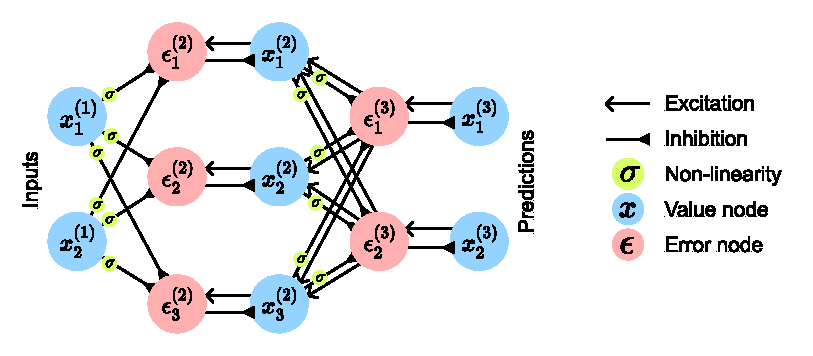
\includegraphics[width=300pt]{graphics/predictive-coding-network.pdf}
  \caption{Predictive coding network with 2 input nodes, 3 hidden nodes and 2 output nodes.}
  \label{fig:predictive-coding-network}
\end{figure}
Predictive coding networks are very similar to feedforward neural networks but include error nodes, $\epsilon_{i,t}^{(l)}$, between value nodes (as illustrated in figure \ref{fig:predictive-coding-network}) that encode the difference between a value node, $x_{i,t}^{(l)}$, and its prediction, $u_{i,t}^{(l)}$:
\begin{equation} \label{eq:pc-error-nodes-and-preds}
  \mathbf{\epsilon}_t^{(l)} = \mathbf{x}_t^{(l)} - \mathbf{u}_t^{(l)},\hspace{10pt}  \mathbf{u}_t^{(l)} = \mathbf{W}^{(l)} \sigma^{(l)}(\mathbf{x}_t^{(l-1)}) + \mathbf{b}^{(l)}
\end{equation}
 Inference learning (IL) is a particular algorithm introduced by Song et al. \cite{PredictiveCodingNetworks} to learn the parameters of predictive coding networks for both supervised and un-supervised learning tasks. The algorithm runs in two phases; an inference phase and a learning phase. To train the network supervised, the input and target nodes are clamped to the input and target variables that the network should learn a mapping between. Then in the inference phase, value nodes are inferred such that they minimize the total free energy of the network:
\begin{equation}
  F_t = \sum_{l=2}^{L}{
    \frac{1}{2}{\lVert \mathbf{\epsilon}_t^{(l)} \rVert}^2.
  }
\end{equation}
To minimize the error nodes, the value nodes are updating according to the following rules;
\begin{equation} \label{eq:update-value-nodes}
  \dot{\mathbf{x}}_t^{(l)} = \begin{cases}
    0 & \text{if } l=1 \\
     -\mathbf{\epsilon}_t^{(l)} + \sigma^{(l)\prime}(\mathbf{x}_t^{(l)}) ( \mathbf{\epsilon}_t^{(l+1)} \mathbf{W}^{(l+1)} )  & \text{if } l = 2 \ldots L-1 \\
    - \mathbf{\epsilon}_t^{(l)} & \text {if } l = L \text{ during prediction} \\
    0 & \text {if } l = L \text{ during learning}
  \end{cases}
\end{equation}
using Eulers method such that $\mathbf{x}_{t+1}^{(l)} = \mathbf{x}_{t}^{(l)} + \gamma \dot{\mathbf{x}}_t^{(l)}$ where $\gamma$ is the integration step size. Once value nodes have converged to an equilibrium at time $t=T$, the parameters are updated to yet again minimize the free energy:
\begin{equation} \label{eq:il-weight-update}
  \Delta \mathbf{W}^{(l)} = \alpha \epsilon_T^{(l)} \sigma(\mathbf{x}_T^{(l-1)}), \hspace{10pt} \Delta \mathbf{b}^{(l)} = \alpha \epsilon_T^{(l)}
\end{equation}
where $\alpha$ is the learning rate. A possible source of confusion when coming from feedforward neural networks is that predictive coding networks do not propagate activity directly from value node to value node. Instead, value nodes should be considered free variables that are updated according to equation \ref{eq:update-value-nodes}. Interestingly, after the inference phase comes to an equilibrium where $\dot{\mathbf{x}}_T^{(l)} = 0$ and all error nodes become zero, the value nodes will correspond to the activity of the neurons in forward prediction of an classic ANN; $0 = \epsilon_{T}^{(l)}=\mathbf{x}_{T}^{(l)}-\mathbf{u}_{T}^{(l)}  \Rightarrow \mathbf{x}_{T}^{(l)} = \mathbf{u}_{T}^{(l)}$, if only the input node is clamped. Even more intriguing is the fact that the error nodes will become approximately equal to the error terms in the back-propagation algorithm (equation \ref{eq:delta-terms}) when both input and output nodes are clamped 
\begin{equation}
    \mathbf{\epsilon}_T^{(L-1)} = \sigma^{\prime}(\mathbf{x}_{T}^{(L-1)})\left(\mathbf{x}_{T}^{(L)} - \mathbf{u}_T^{(L)} \right), \hspace{10pt} \mathbf{\epsilon}_T^{(l)} = \sigma^{\prime}(\mathbf{x}_{T}^{(l)})\left(\epsilon_{T}^{(l+1)} \mathbf{W}^{(l+1)}\right).
\end{equation}
Here, $\mathbf{x}_{T}^{(L)} - \mathbf{u}_T^{(L)}$ is the derivative of the squared loss $\mathcal{L}(y, \hat{y}) = \frac{1}{2}\left( y - \hat{y}  \right)^2$. 


\subsubsection{Z-IL and equivalence to back-propagation}
Song et al. takes this a step further by showing that a special variant of inference learning, zero-divergence inference learning (Z-IL) gives rise to the exact same weight updates as the back-propagation algorithm \cite{PredictiveCodingNetworks}. They show this by first assuming that every value node, $x_{i,t}^{(l)}$ and prediction $u_{i,t}^{(l)}$ is equal to the corresponding forward activity of the equivalent ANN. This is naturally satisfied when the input node is clamped to the input value of some training pair and the network is relaxed to an equilibrium. This corresponds to the forward propagation necessary in back-propagation algorithm. The output node is then fixed to the output value of the training pair after which each value node is updated to minimize $F$ according to equation \ref{eq:update-value-nodes} with integration step size $\gamma = 1$. At last, the weights are scheduled to be updated according to equation \ref{eq:il-weight-update} at time $t=l$.

\subsubsection{Predictive coding networks for classification}
Predictive coding networks by default predict continuous valued output variables and are therefore more suited for regression tasks than classification. However, it is possible to modify the network to perform classification by relying on the insight of deriving the partial derivative of the cross-entropy loss function in section \ref{sec:MLE}. Inference learning updates value nodes in order to minimize the total free energy of the network according to:
\begin{equation}
  \begin{split}
  \dot{\mathbf{x}}_t^{(l)} = -\frac{\partial F_t}{\partial \mathbf{x}_t^{(l)}} & = - \frac{\partial }{\partial \mathbf{x}_t^{(l)}} \left[ \frac{1}{2} {\lVert \epsilon_t^{(l)} \rVert}^2 + \frac{1}{2} {\lVert \epsilon_t^{(l+1)} \rVert}^2  \right] \\
  & = -\epsilon_t^{(l)} - \frac{\partial \frac{1}{2} {\lVert \epsilon_t^{(L)} \rVert}^2}{\partial \mathbf{u}_t^{(l+1)}} \frac{\partial \mathbf{u}_t^{(l+1)}}{\partial \mathbf{x}_t^{(l)}} \\
  & = -\epsilon_{t}^{(l)}+\sigma^{(l+1)\prime}(\mathbf{x}_{t}^{(l)})(\epsilon_{t}^{(l+1)} \mathbf{W}^{(l+1)}).
  \end{split}
\end{equation}
as changing the value node $\mathbf{x}_t^{(l)}$ will both effect its own layers error nodes and error nodes in the next layer as seen in equation \ref{eq:pc-error-nodes-and-preds}. In order for the predictive coding network to perform classification, we set the last weight to the identity matrix, activation function $\sigma^{(L)}(\cdot)$ to the $\softmax$ function and the derivative of the activation function to $\sigma^{(L)\prime}(\cdot) = 1$. We will now consider the second last layer, $L-1$, in the network, corresponding to the logits before being transformed by the softmax function. From the above, the value nodes in the second last layer will now change according to:
\begin{equation}
  \dot{\mathbf{x}}_{t}^{(L-1)} = -\epsilon_{t}^{(L-1)} + \epsilon_{t}^{(L)}.
\end{equation}
Here, we notice that changing $\mathbf{x}_t^{(L-1)}$ in the direction of $\epsilon_{t}^{(L)}$ will actually minimize the cross-entropy loss (as seen in equation \ref{eq:cross-entropy-loss-deriv}), since:
\begin{equation}
  \epsilon_{t}^{(L)} = -\frac{\partial H(\mathbf{x}_t^{(L)}, \mathbf{u}_t^{(L)})}{\partial \mathbf{x}_t^{(L-1)}} = \mathbf{x}_t^{(L)} - \mathbf{u}_t^{(L)}
\end{equation}
Hence, the predictive coding network will learn to perform classification. 
% TODO: Maybe write a little more to this.

\newpage

\section{Results}
\subsection{Experimental Setup}
For all experiments we train classification models in a supervised manner to predict digits in the permutation invariant MNIST task. Each model contains two hidden layer each with 300 neurons. For shadow training SNNs the Adam optimizer is used with a learning rate of $0.0001$ while the PCNs uses SGD with a learning rate of $0.001$. 

\subsection{Experiment 1 - Shadow training spiking neural networks}
\begin{figure}[ht]
  \begin{subfigure}{0.49\linewidth}
    \includegraphics[width=\linewidth]{graphics/spikes_0.png}  
    \subcaption{Neuron activity in the first hidden layer}
  \end{subfigure}
  \hfill
  \begin{subfigure}{0.49\linewidth}
    \includegraphics[width=\linewidth]{graphics/spikes_1.png}  
    \subcaption{Neuron activity in the second hidden layer}
  \end{subfigure}
  \\
  \begin{subfigure}{\linewidth}
    \includegraphics[width=\linewidth]{graphics/spikes-output.png}  
    \subcaption{Output activity of last layer}
  \end{subfigure}
  \caption{Neuron activity in }
\end{figure}


We first use shadow training to train a spiking neural network with LIF dynamics. 


\begin{table}[h]
  \centering
  \begin{tabular}{|l | c|}
  \hline
  \textbf{Model}   & \textbf{Test accuracy} \\ \hline
  Baseline         & 97.68\%                \\
  SNN (Rate-coded) & 97.97\%                \\
  SNN (Spiking)    & 97.71\%                \\ \hline
  \end{tabular}
\end{table}




\section{Discussion}

\section{Conclusion}
\newpage
\bibliographystyle{plain}
\bibliography{refs}


\end{document}
